In diesem Kapitel wird der Versuchsaufbau und die verwendeten Geräte, sowie der Messvorgang erläutert.

\subsection{Versuchsaufbau}

Abbildung \ref{fig:Versuchaufbau} zeigt den in diesem Versuch verwendeten Versuchsaufbau, wie er bei der Michelson Methode üblich ist. Darin ersichtlich sind nebst den zahlreichen Spiegeln, der Laser und der Messokular, sowie die benötigten Streckenangaben.

%%%%%%%%%%%%%%%%%%%%%%%%%%%%%%%%%%%%%%%%%%%%%%%%%%%%%%%%%%%%%%%%%%%%%%%%%%%%%
\begin{figure}[htb]
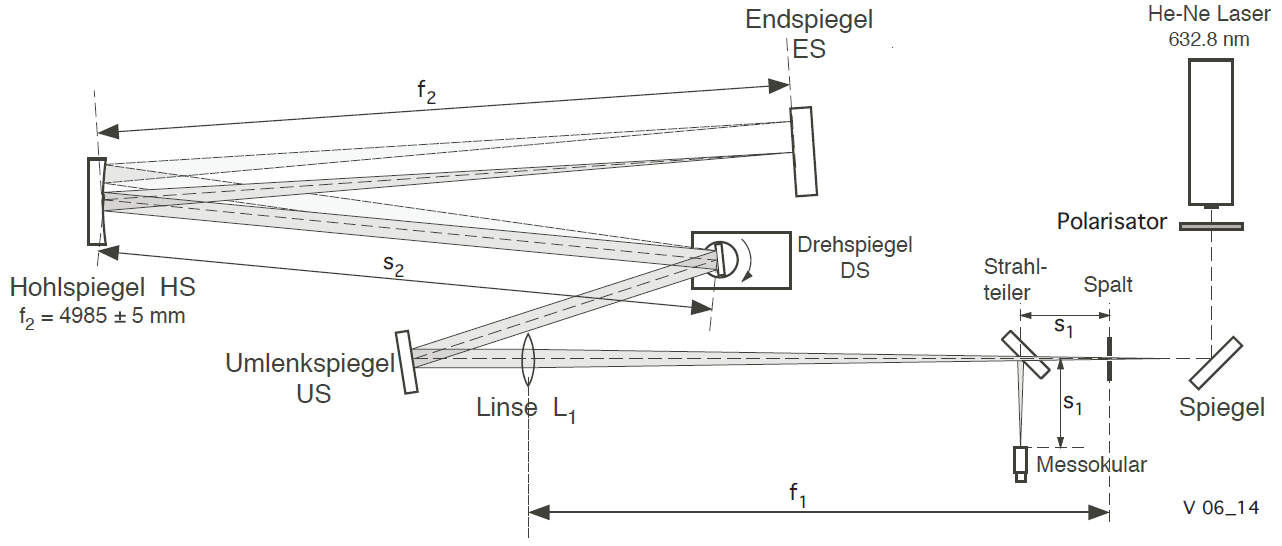
\includegraphics[width=\textwidth]{Messaufbau_Michelson_Grafik.png}
\caption{Versuchsaufbau}
\label{fig:Versuchaufbau}
\end{figure}
%%%%%%%%%%%%%%%%%%%%%%%%%%%%%%%%%%%%%%%%%%%%%%%%%%%%%%%%%%%%%%%%%%%%%%%%%%%%%

\subsection{Messung der Lichtgeschwindigkeit in Luft}

In diesem Unterkapitel werden die verwendeten Geräte, die eingestellten Distanzen, sowie der Messvorgang erläutert.

\subsubsection{Verwendete Geräte}

Nachfolgende Auflistung zeigt alle Geräte die bei diesem Versuch verwendet wurden.

\begin{itemize}
\item Motorspeisung: Power Supply ES030-5
\item Drehfrequenzmessgerät: Pasco OS-9263
\item Laser: 4mW 632 nm
\item Distanzmessung: Leica Disto D8
\end{itemize}

\subsubsection{Eingestellte Distanzen}

Nachfolgende Auflistung zeigt alle für diesen Versuch relevanten Distanzen die eingestellt wurden.

\begin{itemize}
\item Distanz Linse-Spalt ($f_{1}$): $(1\pm 1)m$
\item Distanz Hohlspiegel-Endspiegel ($f_{2}$): $(4.955\pm 1)m$
\item Distanz Strahlenteiler-Spalt und Messokular ($s_{1}$): $(0.12\pm 1)m$
\item Distanz Hohlspiegel-Drehspiegel ($s_{2}$): $(1.075\pm 1)m$
\end{itemize}

\subsubsection{Messvorgang}

Zuerst wurde der Versuchaufbau wie in Abbildung \ref{fig:Versuchaufbau} grob aufgebaut und mit dem durch den Polarisator abgeschwächten Laser kontrolliert. Danach wurden die Distanzen fein eingestellt und die benötigten Distanzen vermessen. Danach wurde eine Drehspiegelfrequenz von 300-400 Hz eingestellt was zu einen leicht verschobenen Beugungsmuster geführt hat. Nach dem Absegnen des Versuchsaufbaus durch den Dozenten wurde dann schliesslich der Drehspiegel auf die gewünschte Drehfrequenz eingestellt und die Okular-Strichmarke auf die markante Stelle des verschobenen Beugungsmusters eingestellt, sodass mittels der Mikrometerschraube der Wert x aus Abbildung \ref{fig:Strahlengang Michelson} abgelesen werden konnte. Diese Messung wurde dann für verschiedene Drehspiegelfrequenzen wiederholt.

\subsection{Äussere Einflüsse}

Da die äusseren Einflüsse wie Temperatur, Luftfeuchtigkeit und Luftdruck eine Rolle spielen für den Wert der Lichtgeschwindigkeit wurden diese Einflüsse während des Versuches gemessen. Die Berechnung des theoretischen Wertes der Lichtgeschwindigkeit $c$ folgt dann im Kapitel \ref{sec:auswertung}.

\begin{itemize}
\item relative Luftfeuchtigkeit: rF = 26\% = 0.26
\item Temperatur: T = 22.3 = 295.45
\item Luftdruck: p = 983hPa = 983 mBar
\end{itemize}